\begin{frame}{Có những nền tảng cơ học giải tích nào?}
    \begin{itemize}
        \item Cơ học Lagrange
        \item Cơ học Hamilton
        \item Cơ học Routhian: kết hợp Lagrange và Hamilton.
        \item Nguyên lý Gauss: Hàm cưỡng bức liên kết tối thiểu.
        \item Phương trình Appell: cho cơ hệ phi Holonom.
        \item Koopman–von Neumann: Cơ học lượng tử cổ điển.
    \end{itemize}
\end{frame}

\begin{frame}{Liên kết Holonomic và phi Holonomic}
\vspace{-4mm}
\begin{columns}
\column{0.5\textwidth}
    \begin{itemize}
        \item\textbf{Liên kết Holonomic}
    \end{itemize}
    \begin{equation}
        f \left( \mathbf{q}, t \right) = 0.
    \end{equation}
    \vspace{-9mm}
    \begin{figure}
        \centering
        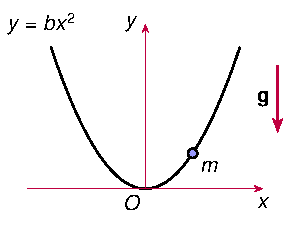
\includegraphics[width=0.8\textwidth]{Figures/Parabol_motion.pdf}
        \vspace{-6mm}
        \caption{Một hạt chuyển động trên bề mặt parabol dưới tác dụng của trọng lực.}
    \end{figure}

\column{0.5\textwidth}
    \begin{itemize}
        \item\textbf{Liên kết phi Holonomic}
    \end{itemize}
    \begin{equation}
        f \left( \mathbf{q}, \dot{\mathbf{q}}, t \right) = 0.
    \end{equation}
    \vspace{-9mm}
    \begin{figure}
        \centering
        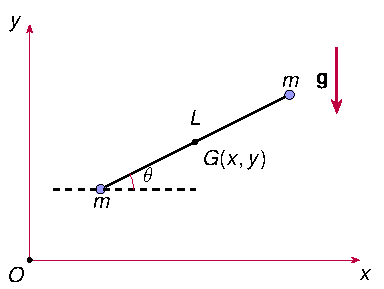
\includegraphics[width=0.8\textwidth]{Figures/NonHolonomic_example.pdf}
        \vspace{-2mm}
        \caption{Một thanh chuyển động dưới tác dụng của trọng trường.}
    \end{figure}
\end{columns}
\end{frame}

\subsection{Cơ học Hamilton}

\begin{frame}{Cơ học Hamilton}

\begin{columns}
\column{0.5\textwidth}
    \begin{itemize}
        \item Biến đổi Legendre: \( H = \sum_{i} p_i \dot{q}_i - L \).
        \item Phương trình Hamilton:
        \vspace{-2mm}
        \begin{align}
            & \dot{q}_i = +\frac{\partial H}{\partial p_i}, \\
            & \dot{p}_i = -\frac{\partial H}{\partial q_i}, \\
            & \frac{\partial H}{\partial t} = - \frac{\partial L}{\partial t}.
        \end{align}
    \end{itemize}
\column{0.5\textwidth}
    \begin{itemize}
        \item Phương trình Hamilton-Jacobi:
        \vspace{-2mm}
        \begin{equation}
            H \left( q_i, \frac{\partial S}{\partial q_i}, t \right) + \frac{\partial S}{\partial t} = 0.
        \end{equation}
        \item Liên hệ trực tiếp với hàm tác dụng \(S\)
        \begin{equation}
            p_i = \frac{\partial S}{\partial q_i}.
        \end{equation}
    \end{itemize}
\end{columns}
\end{frame}

\subsection{Nguyên lý Gauss về liên kết tối thiểu}

\begin{frame}{Nguyên lý Gauss}

\begin{columns}
\column{0.5\textwidth}
    \textbf{Độ cưỡng bức}
    \begin{equation}
        Z = \frac{1}{2} \sum_{i=1}^{N} m_i \left| \mathbf{a}_i - \frac{\mathbf{F}_i}{m_i} \right|^2.
    \end{equation}
    đạt cực tiểu (tức là \(\delta Z = 0, \delta^2 Z > 0\)).

    \textbf{Ví dụ:} \( Z = m \left[ \left( \ddot{x} \right)^2 + \left( \ddot{y} + g \right)^2 \right]\).
    \vspace{-2mm}
    \begin{align}
        & \delta \ddot{y} = 2 b x \delta \ddot{x} \\
        & \delta Z = 2m \left( \ddot{x} \delta \ddot{x} + \left( \ddot{y} + g \right) \delta \ddot{y} \right) = 0 \\
        & \Rightarrow \ddot{x} + 2b x \left( \ddot{y} + g \right) = 0 \\
        & \Rightarrow \left( 1 + 4 b^2 x^2 \right) \ddot{x} + 4 b^2 x \dot{x}^2 + 2 b x g = 0.
    \end{align}

\column{0.5\textwidth}
    \vspace{-6mm}
    \begin{figure}
        \centering
        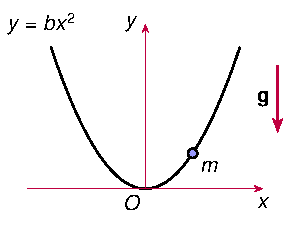
\includegraphics[width=0.9\textwidth]{Figures/Parabol_motion.pdf}
        \vspace{-2mm}
        \caption{Chuyển động của một hạt trên rãnh parabol dưới tác dụng của trọng lực.}
    \end{figure}
\end{columns}

\end{frame}

\subsection{Phương trình Appell cho cơ hệ phi Holonom}

\begin{frame}{Phương trình Appell cho cơ hệ phi Holonom}

\begin{columns}
\column{0.5\textwidth}
    \vspace{-3mm}
    \textbf{Năng lượng gia tốc}
    \begin{equation}
        S = \frac{1}{2} \sum_{i=1}^{N} m_i \left| \ddot{\mathbf{r}}_i \right|^2.
    \end{equation}

    \textbf{Ví dụ:} \( S = m \left[ \ddot{\pi}^2 + L^2 \left( \ddot{\theta}^2 + \dot{\theta}^4 \right) \right] \) 
    với á vận tốc: \( \dot{\pi} = \dot{x}/ \cos ( \theta ) = \dot{y}/ \sin ( \theta )\).

    Biến phân công: \(\delta A = Q_{\pi} \delta \pi + Q_{\theta} \delta \theta\)
    với \( Q_{\pi} = -2 mg \sin ( \theta ), Q_{\theta} = 0\).

    Phương trình Appell
    \vspace{-2mm}
    \begin{align}
        & \frac{\partial S}{\partial \ddot{\pi}} = Q_{\pi}, \quad \frac{\partial S}{\partial \ddot{\theta}} = Q_{\theta} \\
        & \Rightarrow m \ddot{\pi} = -2 mg \sin ( \theta ), \quad m L^2 \ddot{\theta} = 0.
    \end{align}

\column{0.5\textwidth}
    \vspace{-6mm}
    \begin{figure}
        \centering
        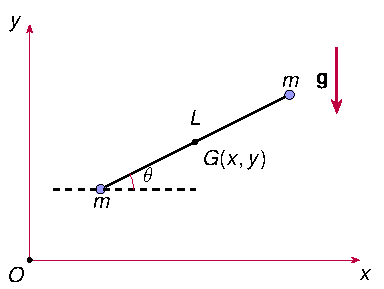
\includegraphics[width=0.9\textwidth]{Figures/NonHolonomic_example.pdf}
        \vspace{-2mm}
        \caption{Một thanh chuyển động dưới tác dụng của trọng trường.}
    \end{figure}
\end{columns}
    
\end{frame}